
\section{Earth Centered Earth Fixed Coordinates ECEF } \label{sec:itrf} 
Within JEOD Earth centered Earth fixed coordinates are referred to as ECEF.
This is a heritage nomenclature. Body fixed coordinates are the frame in which a non-spherical gravitational field is defined. There exist within JEOD the fields GEM-T1 and GGM02C, the first is defined with respect to the ECEF frame, GGM02C uses the International Terrestrial Reference Frame frame. (One notes these frames have only small difference at the Epoch date of J2000.)
ITRF is realized by the locations of a set of points or stations on a tide-free Earth. As measurements and models have improved or changed, these locations have been changed also and the ITRF moves slightly with respect to the physical Earth every few years.
For details see the IERS specification document \cite{IERS2003}. The ITRF system is related to the ICRF system by the Earth orientation model realized by the JEOD \RNP.
Note the body fixed coordinate states can be recorded but cannot be used to initialize a simulation.

\textbf{Coordinate Frame: } Rotating

\begin{itemize}
\item X-axis: The intersection of the prime meridian and the rotation equator of the Earth.
\item Y-axis: Completes a standard, right-handed coordinate frame.
\item Z-axis: The rotation pole of the Earth.
\end{itemize}

\begin{figure}[htp]
\centering
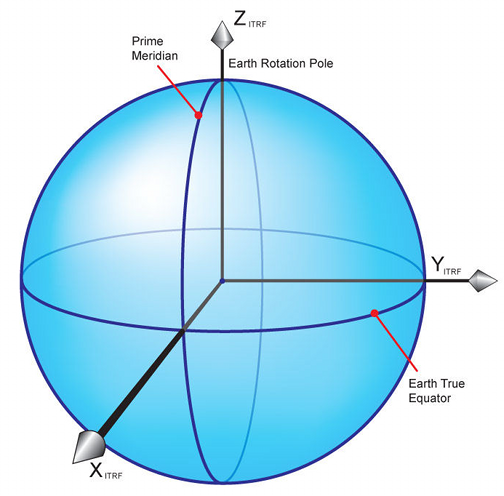
\includegraphics [width=7in]{figs/fig5.png}
\caption{International Terrestrial Reference Frame}
\label{fig:5}
\end{figure}

\subsection{Example ECEF}
See the example in Section 4 \ref{sec:icrf}.
In the Tutorial simulation SIM 2 is an example of recording Earth planet fixed coordinates. 
\begin{verbatim}
earth.planet.pfix.state.rot.T_parent_this[0][0-2]
earth.planet.pfix.state.rot.T_parent_this[1][0-2]
earth.planet.pfix.state.rot.T_parent_this[2][0-2]
\end{verbatim}

